\chapter{Modeling of random alloys}
\label{sec:SQS}

The structure of high-entropy alloys in which the alloying elements occupy lattice sites by a random probability pose a problem on the numerical methods used for modeling. DFT in particular rely heavily on the periodicity in crystalline solids, as we will discover later. 
In a brute force approach, this could be solved by randomly distribute the solute and solvent atoms over the lattice sites of a large supercell and average the energy and related properties of a great number of such supercells with varying distributions. Obviously this approach is rather efficient or even doable considering the computational demand. Thankfully today there exists a number of possible methods to more efficiently study such structures. Examples are the virtual crystal approximation (VCA), Coherent Potential approximation (CPA), special quasi-random structure (SQS), and hybrid monte-carlo/molecular dynamics. (MC/MD). A brief review of the different models is given in for example \cite{sqsIntro}. In this project we will employ the SQS method, due to both it's easy to use implementation and interpretation in VASP compared to the other options, and other benefits that will become clear after the following sections.             

\section{The Special Quasi-random Structure model}
In the original paper on SQS published in 1990 \cite{sqsfull}, it was proposed a selective occupation strategy to design special periodic quasi-random structures that exceeded previous methods in both accuracy and cost. The key concept was to create a periodic unit cell of the various components in a finite N lattice site single configuration such that the structure most closely resemble the configuration average of an infinite perfect random alloy. In an attempt to work withing the 50 lattice sites boundary of ab initio methods at that time. The working theory was that if one can resemble an infinite perfect random alloy by a periodic finite N cell, also the electronic properties would be similar between the two. The solution to this model was that for each N, ie lattice site, to minimize the difference of structural correlation function between the approximated cell and the perfect random alloy. There are obviously errors involved with approximating a random alloy by a periodic cell, but by the hierarchical relation to the properties of the material, interactions between distant sites only offer a negligible small contribution to the total energy of the system. Thus the aim of the SQS method is focused around optimizing the correlations within the first few shells of a given site. To follow is a review of the mathematical description of special quasi-random structures.

\subsection{Mathematical description}
We begin this section by giving a brief review of topics such as cluster expansions, statistics and superposition of periodic structures. A broader description of these topics can be found in the original article, or elsewhere in the literature. On a side note regarding the following mathematical derivation, the original concept was devolved in mind of an random binary alloy, but the theory have late successfully been extended to multi-component alloys and other special cases. 

The different possible atomic arrangements are denoted as "configurations" $\sigma$. The various physical properties of a given configuration is $E(\sigma)$, and $<E>$ is the ensemble average over all configurations $\sigma$. In practice, this quantity is unfeasible in terms of computational cost, seeing as the average require calculations and relaxations of all possible configurations, for a binary alloy this is $2^N$ for a fixed N number of lattice sites. A solution to this is to use the theory of cluster expansions and discretize each configuration into "figures" $f$. A figure in the lattice is defined in terms of the number of atoms it include $k$, distance in terms of neighbors $m$, and position in the lattice $l$. Further we assign spin values for each lattice site $i$ in the figure to denote which element it holds (+1,-1 for a binary alloy). By defining the spin product of spin variables in a figure at lattice position $l$ as $\Pi_f(l, \sigma)$, we can write the average of all locations in the lattice of a given figure $f$ as 
\begin{equation}
    \boldsymbol{\Pi}_f(\sigma) = \frac{1}{ND_f} \sum_l \Pi_f (l,\sigma)
\end{equation}
where $D_f$ is the number of equivalent figures $f$ per site. The brilliance of this notation is that we now can express the physical property $E(\sigma)$ in terms of the individual contributions $\epsilon_f$ of a figure f.
\begin{equation}
    E(\sigma) = \sum_{f,l} \Pi_f(l, \sigma) \epsilon_f(l)
\end{equation}
The quantity $\epsilon_f$ is called the "effective cluster property" and is defined as (for a random binary alloy $A_{1-x}B_x$)
\begin{equation}
    \epsilon_f(l) = 2^{-N}\sum_\sigma^{2^N} \Pi_f (l,\sigma) E(\sigma)
\end{equation}
Inserting the equation for $\boldsymbol{\Pi}_f$ into that of $E(\sigma)$ we can describe the the previous cluster expansion of $E(\sigma)$ as
\begin{equation}
    E = N\sum_f D_f<\boldsymbol{\Pi_f}>\epsilon_f
\end{equation}
And obtain a simplified expression for $<E(\sigma>)$ in eq 1? Thus we have successfully managed to reduce the expensive task of sampling all $E(\sigma)$ into calculating the effective cluster properties and summing over all types of figures. Remembering that $E(\sigma)$ can relate to many physical properties, the most common and applied case is that $E(\sigma)$ is the total energy, while $\epsilon_f$ is many body interaction energies. The cluster expansion above converge rather quickly with increasing number of figures, an effective method is thus to select a set of configurations to evaluate the effective cluster properties. Don't know how to write this, but the next step is to select a finite largest figure denoted $F$, and "specialize" the cluster expansion to a set of $N_s$ periodic structures ${\sigma} = ${s} to obtain the two expressions for $E(s)$ and $\epsilon_f$ using matrix inversion to obtain the result for $\epsilon_f$
\begin{align}
E(s) &= N\sum_{f}^{F} D_f \boldsymbol{\Pi}_f (s)\epsilon_f \\     
\epsilon_f &= \frac{1}{ND}\sum_{s}^{N_s}[\boldsymbol{\Pi}_f (s)]-1E(s)
\end{align}
Assuming now that the sum of figures $F$ and $N_s$ periodic structures are well converged, $E(\sigma)$ can be rewritten as a superposition of $E(s)$
\begin{align}
    E(\sigma) &= \sum_{s}^{N_s}\xi_s(\sigma)E(s) \\
    \xi_s(\sigma) &= \sum_{f}^{F}[\boldsymbol{\Pi}_f(s)]^{-1}\boldsymbol{\Pi}_f(\sigma)    
\end{align}
where $\xi$ is the weights. Thus we have effectively reduced the problem to a convergence problem of the number of figures $F$ and structures $N_s$. This can be easily solved given that we are dealing with periodic crystal structures ${s}$ that can employ the general applications of ordered structures from ab initio methods, and increasing $F$ until the truncation error falls bellow a desired threshold. However, this approach requires that the variance of the observable property is much lower than the sample mean, otherwise one would have to employ a much bigger sample size to reach statistical convergence. Don't how to write this part nicely, but: Because of the different relationship between various physical properties and the correlation functions, one observe different convergence depending on the meaning of $E$. The idea behind SQS was therefore to design single special structures with correlation functions ${\boldsymbol{\Pi}_f(s)}$ that most accurately match those of the ensemble average of a random alloy $<\boldsymbol{\Pi}_f>_R$. 

The correlation functions of an perfect random infinite alloy, denoted as $R$ is defined bellow
\begin{equation}
    \boldsymbol{\Pi}_{k,m}(R) = <\boldsymbol{\Pi}_{k,m}>_R = (2x-1)^l 
\end{equation}
with $k, m$ defined as before and x being the composition ratio of the alloy. In the case of an eqvimolar alloy ($x=\frac{1}{2}$), the functions equal 0 for all $k$ except $<\boldsymbol{\Pi}_{0,1}>_R = 1$. If we now randomly assign either atom A or B to every lattice site, for a sufficiently large value of N, the goal is then to create a single configuration that best match the random alloy. Keeping with the $x=\frac{1}{2}$ case, the problem is now that even though the average correlation functions of a large set of these structures approaches zero, like for the random alloy. The variance of the average is nonzero meaning that a selected structure of the sample is prone to contain errors. The extent of these errors can be evaluated from the standard deviations
\begin{equation}
    \nu_{k,m}(N) = |<\boldsymbol{\Pi}^{2}_{k,m}>|^{\frac{1}{2}} = (D_{k,m}N)^{-\frac{1}{2}}
\end{equation}
Given the computational aspects, it's obvious that economical structures with small N are prone to large errors. In fact, in some cases these errors can result in correlation functions centering around 1, as opposed to 0 for a perfect random alloy.  

I don't know how to write the prelude to this part! (see section IIIA in \cite{sqsfull}). The degree to which a structure $s$ fails to reproduce the property $E$ of the ensemble-averaged property of the random alloy can be described by a hierarchy of figures, see eq .. bellow
\begin{equation}
    <E> - E(s) = \sum_{k,m}' D_{k,m}[(2x-1)^k-\boldsymbol{\Pi}_{k,m}(s)]\epsilon_{k,m}
\end{equation}
, the prime is meant symbolize the absence of the value $0,1$ for $k,m$. The contribution from the figure property $\epsilon$ reduces for larger figures. In general, for disordered systems, the physical property "E" at a given point R falls of exponentially as $|R-R'|/L$, where L is a characteristic length scale relating to the specific property. Using this, the approach of SQS is to specify a set of correlation functions that hierarchically mimic the correlation functions of the random alloy. Meaning that it prioritize the nearest neighbor interactions. With the set of functions decided on, the objective it finally to locate the structures that correspond to the selected structures. 

With this approach, \cite{sqsfull} managed by mimicking the correlation functions exact for the first two shells, to reduce the computational measures of an accurate models. In this exact study they matched the results of an $N \rightarrow \infty$ by an $N=8$ SQS. In the final section of this chapter, we will take a look at the recent advances in the SQS method and application to high-entropy alloys. 

\subsection{Applications to high-entropy alloys}
The success of the SQS method is in large part related to to the fact that we can create simple periodic structures, this allows for the use of standard DFT methods to calculate with ease properties such as the total energy, charge density and electronic band structure \cite{sqs_dos}, \cite{sqs_bg}. However, some certain obstacles arise when trying to apply the SQS model to high-entropy alloys. An exhaustive analysis discussing several of these factors and comparing to alternative methods were performed in 2016 by M.C Gao et al. \cite{hea2016_ch10}  in the framework of DFT and VASP.

The first initial concern is the size of the supercell. This parameter  needs to be balanced between accuracy and cost. A larger SQS cell consisting of a greater number of atoms better encapsulate the disordered structure of HEAs, but both the generation and simulation of such large SQSs come at an increased computational demand.  M.C Gao discovered a significant sensitivity between the registered stability and predicted crystal structure of \ch{CoCrFeNi} and \ch{CoCrFeMnNi} HEAs and varying SQSs sizes. Experimentally both of these is found stable in the FCC structure. By calculating the enthalpy of formation, he found that SQSs under 64 atoms wrongly predicted the HCP structure as the most stable, while larger SQS correctly agreed on the FCC structure. Additionally, the probability distribution functions (PDFs) of the respective SQSs display a dependence to the SQS size. For example in 3 SQSs of size 20, 125 and 250 atoms each of FCC CrFeMnNi, the Cr-Mn is much better represented in the large SQS model as seen bellow in figure 4.1.

\begin{figure}[H]
\begin{subfigure}{.5\textwidth}
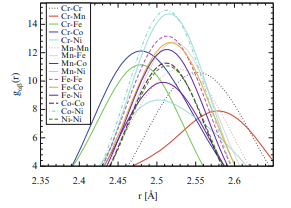
\includegraphics[width=\textwidth]{theory/PDF_small.png}
\caption{20 atom SQS}	
\end{subfigure}
\begin{subfigure}{.5\textwidth}
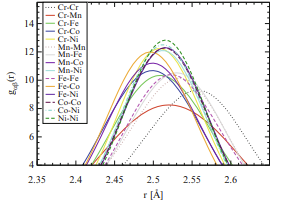
\includegraphics[width=\textwidth]{theory/PDF_big.png}
\caption{250 atom SQS}
\end{subfigure}
\caption{PDFs of (a) 20 and (b) 250 atom SQS models of CrFeMnNi \cite{hea2016_ch10}}
\end{figure}
     
It can also be noted that a similar dependence on the SQS size is apparent for the entropy and mechanical properties, however these topics are not relevant for this project and will thus not be elaborated further. Bellow we summarize the findings of M.C Gao et al between the SQS model and the crystal potential approximation and hybrid monte-carlo/molecular dynamics applied to high-entropy alloys. The comparison of SQS and MC/MD in terms of the calculated density of states can be seen in figure 3.2.
      
\begin{figure}[H]
\centering
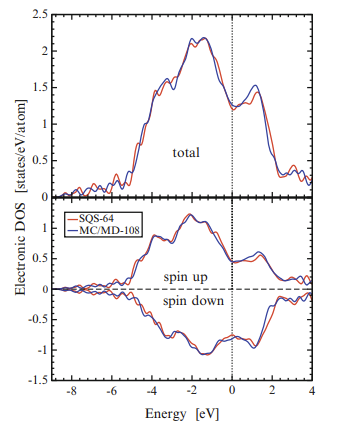
\includegraphics[width=.6\textwidth]{theory/SQS-MCMD_DOS.png}
\caption{Density of states with SQS and MC/MD of FCC CoCrFeNi, figure from \cite{hea2016_ch10}}
\end{figure}

The density of states (DOS) of the MC/MD simulations were conducted on a larger 108 atom cell, compared to a 64 atom SQS. In despite of both the larger cell and much more complex calculations, the results of the SQS model measures up well. Furthermore, the SQS model produce a comparative outcome of the probability distribution functions (PDFs) to MC/MD as seen bellow. 

\begin{figure}[H]
\centering
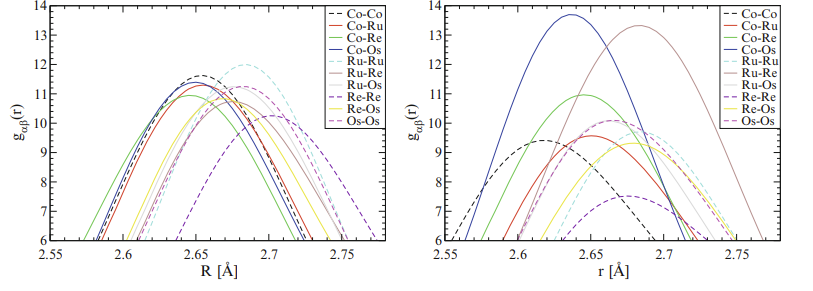
\includegraphics[width=\textwidth]{theory/SQS-MCMD_PDF.png}
\caption{Probability distribution functions with SQS and MC/MD of HCP CoOsReRu \cite{hea2016_ch10}}
\end{figure}

The discrepancy in the PDFs are seen as more accurate from MC/MD calculations compared to experimental values. This is because SQS fail to include inter-atomic interaction and preference to the same extent as MC/MD. This is illustrated in figure 3.3 for the HCP CoOsreRu alloy, in which clear preference of Co-Os and Re-Ru pairs is apparent from MC/MD simulations but not in the SQS model. Regardless, the results of SQS is very good considering the simplicity of the model and implementation. Compared to the CPA method, SQS is the less equipped method for dealing with specific cases such as \ch{A{1/3}BCDE} structures, and paramagnetic materials \cite{hea2016_ch10} 

We have seen up until this point that the SQS method utilized an intelligent approach which allows for a simple implementation and calculations while providing results mostly on par to other more intricate and complex solutions to model disordered structures. However one particular factor concerning SQS that does not apply for CPA and MC/MD, is that within the SQS model one material can obtain in a number of distinct configurations. For example a quaternary and quinary alloy make for 24 and 124 unique configurations respectively, resulting in an uncertainty of the energy regarding the different permutations. This effect is most prominent in anisotropic lattices such as HCP and alloys with chemically dissimilar constituents, and particularly in small SQS cells \cite{hea2016_ch10}. 

 
Despite of it's flaws, especially in recent years SQS have emerged as a viable and trusted method of modeling disordered structures such as HEA. This is down to both the increasingly available computational power and improvements to the SQS method. The latter particularly saw a boost in 2013 with the introduction of the MC-SQS method \cite{mcsqs2013}, short for Monte-Carlo Special Quasirandom Structures. Contrary to the original SQS method that seek to minimize the difference between the correlation functions of the approximated cell and the true random alloy, this method employ monte-carlo simulations to perfectly match a maximum number of correlation functions. Furthermore emphasizes an efficient and fast implementation in addition to an exhaustive unbiased search of possible atomic configurations. Following, this is the preferred and most widely used method of choice in today's research, specific details on the method can be found in \cite{mcsqs2013}. \textbf{How much detail do I need to include here, should I do a full explanation of the method or does this suffice?}  This has resulted in an increased number of studies utilizing SQSs to investigate high-entropy alloys \cite{WANG2021128754}, \cite{WEI2021167432}, \cite{RASHID2014285}, and \cite{SORKIN2021160776}.   






























































